\chapter{Data Collection}
\label{sec:Data_Collection}

The data collection portion of this project is immediately tasked with the following set of problems: spatial coincidence, temporal coincidence, and resolution. Given the asynchronous orbits of each satellite and the incompatible resolutions of ESA's SN-2 and NASA's IS-2, other avenues were explored to obtain precise SAR imaging. Of note were NASA's "ICESAT-2" mobile application and ICEYE's\textsuperscript{\tiny\textcopyright} SAR imaging offered through the ESA. The ICESAT-2 mobile application tracks IS-2's footprint location and lists the dates and times of when the satellite will next fly over a position. ICEYE is a third party satellite provider through the ESA that offers "SPOT" and "SLEA" SAR imaging products, featuring 1m resolution and extent ranging from 1km$^2$ to 15km$^2$ \cite{iceye-products}. The appeal of ICEYE's 1m resolution products is that a nominal acquisition of its SPOT data product would coincide with $\approx$350 unique IS-2 footprints while the SLEA product would coincide with $\approx$5300.

\section {SAR Imaging}
ICEYE's superior resolution is significantly more compatible with IS-2's small footprint, but is not made freely available as it's a private company. However, they are a participant in the ESA's Third Party Missions Program, meaning the ESA can sponsor the data delivery through their Earth Observation User Services Portal. 

To achieve ESA sponsorship of this data, a proposal was submitted including the objective of the project, researchers involved in the task, which satellite and product was being requested, and a general plan outlining the use of the sponsored data. Given the latency of proposal approval, and the seasonal characteristics of arctic sea ice, interim efforts were made to coincide freely available SN-2 10m resolution data with IS-2's altimetry.

\begin{figure}[h]
    \centering
	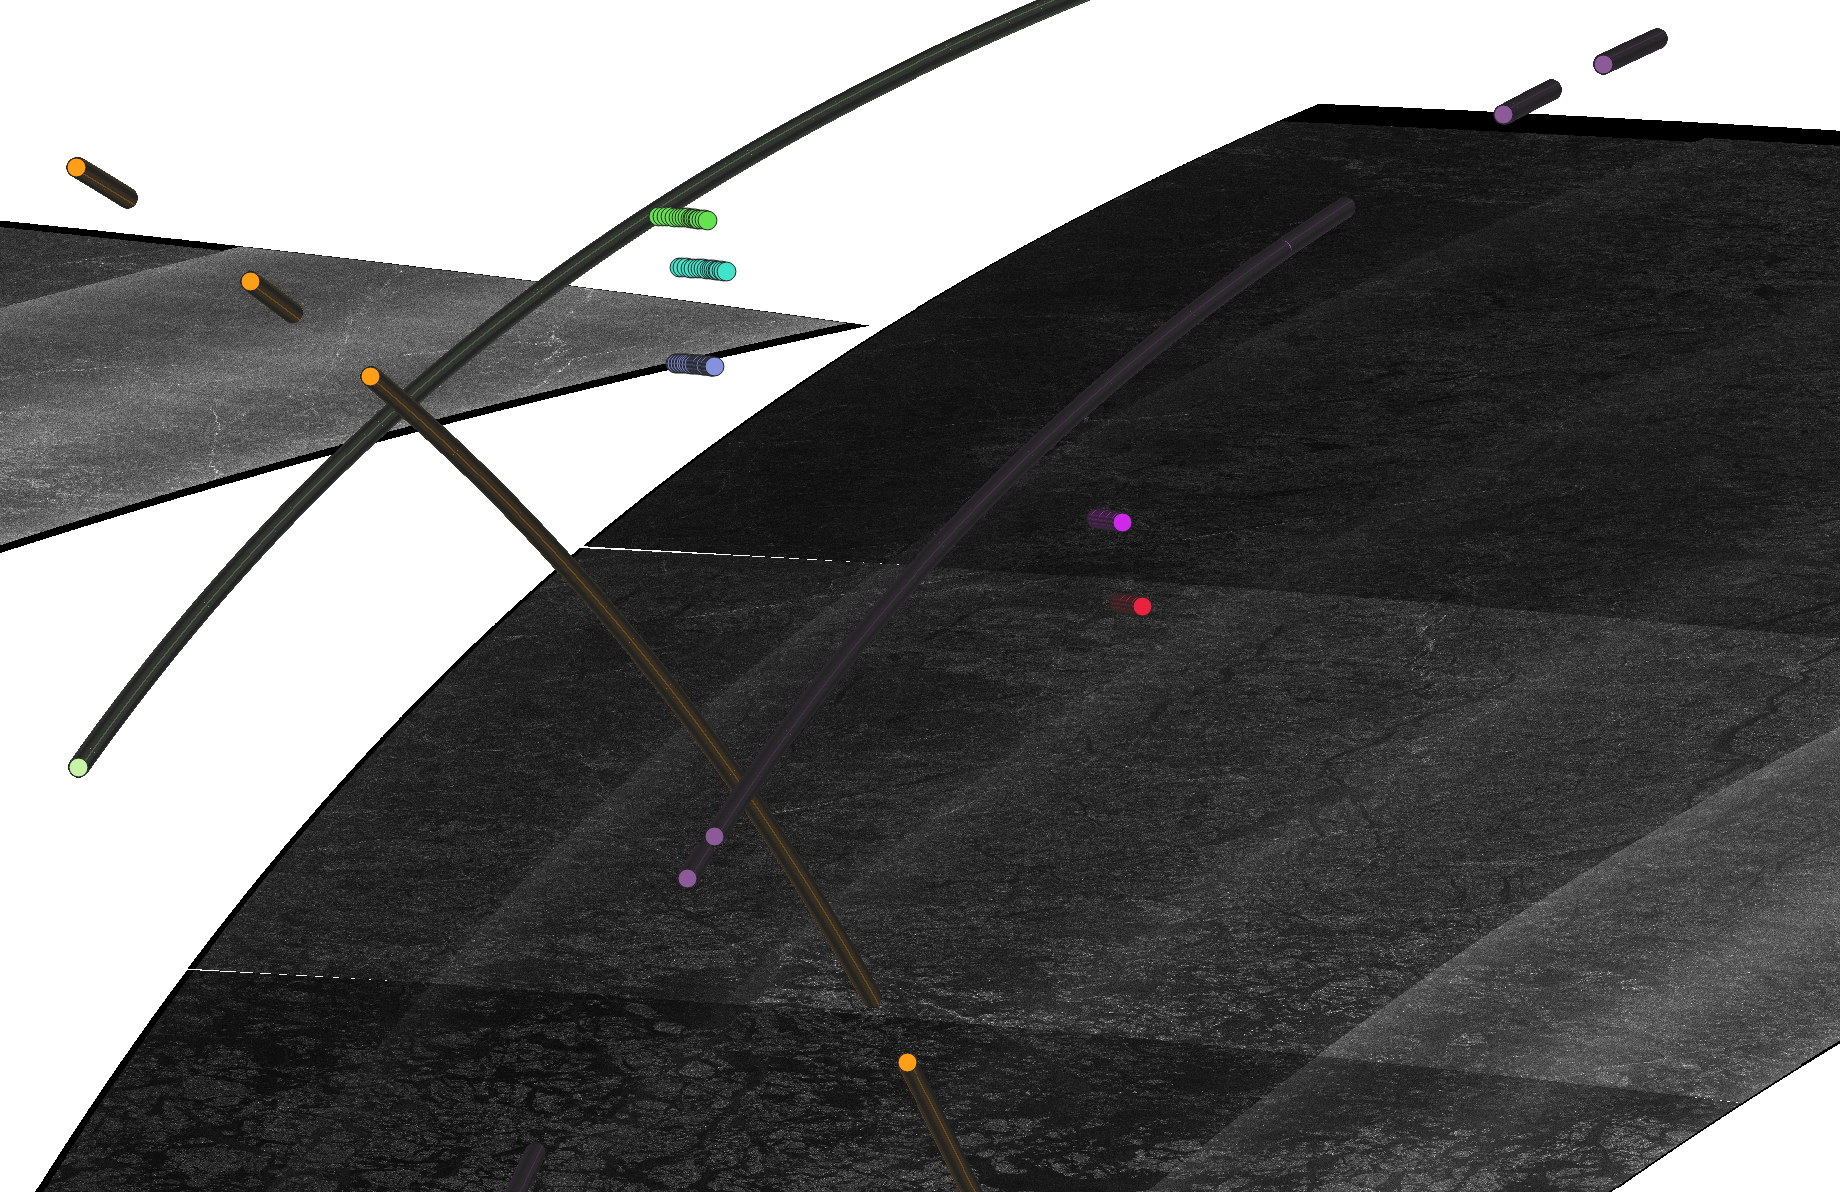
\includegraphics[width=.8\textwidth]{../research-resources/ice-sat-2/near-coincidence-buoys.png}
    \caption[Existing Coincident Data Unavailability]{Near-Coincidence of SN-2 and IS-2, February 20-21 2023}
    \label{fig:near-coincidence}
\end{figure}

Referring to ESA's Copernicus Open Access Hub and NASA's Earthdata Search tool, a near coincident set of SN-2 and IS-2 data was obtained for February 20-21 of 2023 (Figure \ref{fig:near-coincidence}). The SAR imaging clearly captured regions of arctic ice, and did so on February 20th at 4:50pm UTC. The predominantly spatially coincident IS-2 measurements, being the long purple and orange tracks in the figure, crossed the region at 10am and 10pm UTC on February 21. This data while immensely geographically coincident, was dubious because of its 17 and 29 hour respective temporal delay. Utility scripts were devised to track buoy movement in the area across the time period, and the nearest buoy (purple) to any of the tracks was 30 kilometers away and had traveled another 8 km during the data's time difference. The corroboration of buoy movement in the area invalidates the possibility of the data being correlated, as it's unreasonable to account for the drift of the ice over the given time and space scale. While unsuccessful, this instance demonstrates the unavailability of naturally coincident data and the inefficiencies in obtaining it.

Later, the ESA approved the project proposal and agreed to sponsor 2 SPOT and 2 SLEA images. With this sponsorship, specific SAR imagery was then ordered that coincided with IS-2's flight path. In preparation for the data order, locations were selected in the ICESAT-2 mobile application and validated to have sea ice by viewing recent SN-2 data via Copernicus Open Access Hub. Then, an order form was submitted to ICEYE detailing the acquisition information to which they'd respond regarding its feasibility. This ordering and validation was repeated until all 4 sponsored images were fulfilled (Figure \ref{fig:gathered-sar}).

\begin{figure}[h!]
    \centering
    \subfigure[]{\includegraphics[width=.48\linewidth]{./research-resources/SAR/ICEYE_X13_QUICKLOOK_SLEA_3279210_20240119T023534.png}\label{fig:gathered-sar-a}}
    \subfigure[]{\includegraphics[width=.48\linewidth]{./research-resources/SAR/ICEYE_X2_QUICKLOOK_SLEA_3279211_20240119T044029.png}\label{fig:gathered-sar-b}}
    \subfigure[]{\includegraphics[width=.48\linewidth]{./research-resources/SAR/ICEYE_X6_QUICKLOOK_SLH_3280232_20240120T132858.png}\label{fig:gathered-sar-c}}
    \subfigure[]{\includegraphics[width=.48\linewidth]{./research-resources/SAR/ICEYE_X8_QUICKLOOK_SLH_3295462_20240120T202547.png}\label{fig:gathered-sar-d}}
    \caption[ICEYE Captured SAR Imagery]{
    \\\hspace{\textwidth}
    (a) SLEA 1/19 02:35:35 UTC (73.396, -141.668)\\\hspace{\textwidth}
     (b) SLEA 1/19 04:40:35 UTC (73.395, -141.664),\\\hspace{\textwidth}
      (c) SPOT 1/20 13:29:02 UTC (72.816,-133.975),\\\hspace{\textwidth}
      (d) SPOT 1/20 20:25:52 UTC (72.816, -133.976)
      }
    \label{fig:gathered-sar}

\end{figure}

\section {Laser Altimetry (IceSat-2)}
The ICESAT-2 mobile application and ICEYE's flexibility handled the issues of spatial and temporal coincidence. IS-2 data was simply collected from the National Snow and Ice Data Center (NSIDC) repository after its own acquisition of the selected area. Each IS-2 acquisiiton offers multiple data products, but for the study of sea ice the ATL10 product is most relevant. The ATL10 data product contains inferences about sea-ice freeboard using data propagated from the separate ATL07 sea ice height product. Thus, a single ATL10 delivery contains the interpreted sea surface height, ice surface height, and the total freeboard \cite{ICESat-2-ATL10-Product} needed to infer sea ice thickness (Equation \ref{eq:isostatic-equilibrium}).

The recorded data is captured and delivered in a ".h5" file requiring parsing to extract relevant information. Appendix A contains a list of the fields that were extracted, and a brief description of each based upon the ATL10 data product specification \cite*{ICESat-2-ATL10-Product}.

After receiving the SAR imaging from ICEYE and the IS-2 data from the NSIDC, the best delivery in terms of coincidence was Figure \ref{fig:gathered-sar-b}. Figure \ref{fig:gathered-sar-b} was 6 minutes coincident with the IS-2 track, thus offering the greatest source of ground truth. A severe limitation of the extracted data though, is that IS-2 omits data when it detects ice concentration $<$50\%. For this reason, the ATL10 .h5 product for this acquisition only contained data from its GT2R and GT3R beams, effectively yielding 33\% of the information initially expected. Figure \ref{fig:icesat2-tracks} shows the intersecting IS-2 tracks, and Figure \ref{fig:ice-thickness-gathered} demonstrates the surface profile of the captured data, which will be used to interpolate ice thickness in future sections.


\begin{figure}[h!]
	\centering
	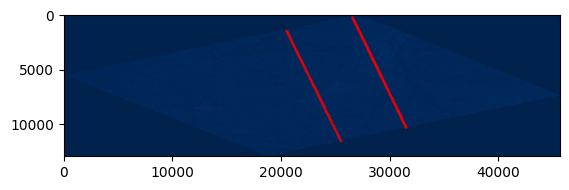
\includegraphics[width=\textwidth]{../research-resources/ice-sat-2/icesat2-tracks.png}
	\caption[Overlayed LiDAR and SAR Readings]{IS-2 Tracks across ICEYE Image}
	\label{fig:icesat2-tracks}
\end{figure}

\begin{figure}[h!]
	\centering
	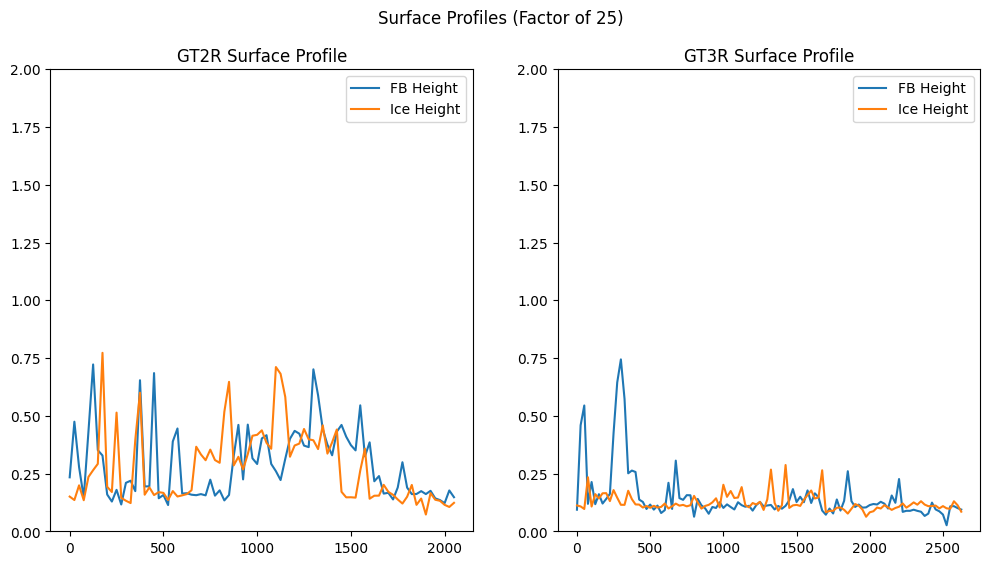
\includegraphics[width=\textwidth]{../research-resources/ice-sat-2/Surface Profiles.png}
	\caption[Ice Surface Profile of Acquired Data]{Ice Surface Profiles}
	\label{fig:ice-thickness-gathered}
\end{figure}

